	\documentclass[a4paper,12pt,twoside]{scrreprt}
% nezbytné balíčky
\usepackage[T1]{fontenc}
\usepackage[utf8]{inputenc}  % vstupní znaková sada: UTF8
\usepackage[czech]{babel} % typografická pravidla     
\usepackage[a4paper, hmarginratio=3:2]{geometry} % využití celé A4 stránky a nastavení okrajů
\usepackage{graphicx} % balíček pro vkládání obrázků
\usepackage{tabularx} % rozšířené možnosti tabulek
\usepackage{indentfirst}
\usepackage{titlesec} 
\usepackage{amsmath}
\usepackage{listings}

% balíčky, které se mohou hodit
%\usepackage{amsmath} % balíček pro pokročilou matem. sazbu
%\usepackage{color} % pro možnost barevného textu
%\usepackage{fancybox} % umožňuje pokročilé rámečkování
%\usepackage{index} % nutno použít v případě tvorby rejstříku balíčkem makeindex
%\newindex{default}{idx}{ind}{Rejstřík} % zavádí rejstřík v případě použití balíku index
%\usepackage{caption} % pro popisky obrázků, tabulek atd.
%\usepackage{listings}  % balíček vhodný pro ukázky kódu 
%\usepackage{float} % rozšířené možnosti umístění obrázků
%usepackage[hidelinks]{hyperref} % pro klikací odkazy v pdf
%\usepackage{encxvlna} % postará se o spojky a předložky, které dle českých pravidel nesmí být na konci řádku. Dokumentace: http://texdoc.net/texmf-dist/doc/generic/encxvlna/encxvlna.pdf


% spacing: how to read {12pt plus 4pt minus 2pt}
%           12pt is what we would like the spacing to be
%           plus 4pt means that TeX can stretch it by at most 4pt
%           minus 2pt means that TeX can shrink it by at most 2pt
%       This is one example of the concept of, 'glue', in TeX
%		\titlespacing{command}{left spacing}{before spacing}{after spacing}[right]

\titlespacing{\section}{0pt}{\parskip}{-\parskip}
\titlespacing{\subsection}{0pt}{\parskip}{\parskip}
%\titlespacing{\subsubsection}{0pt}{\parskip}{-\parskip}

%\titlespacing\chapter{0pt}{0pt plus 2pt minus 2pt}{0pt plus 0pt minus 0pt}
%\titlespacing\section{0pt}{0pt plus 0pt minus 0pt}{0pt plus 0pt minus 0pt}
%\titlespacing\subsection{0pt}{2pt plus 4pt minus 2pt}{0pt plus 0pt minus 0pt}
%\titlespacing\subsubsection{0pt}{12pt plus 4pt minus 2pt}{0pt plus 2pt minus 2pt}

\topmargin=-15mm      % horní okraj trochu menší
\textwidth=150mm      % šířka textu na stránce
\textheight=240mm     % "výška" textu na stránce

\pagenumbering{arabic} % číslování stránek arabskými číslicemi
\pagestyle{plain}      % stránky číslované dole uprostřed

\parindent=22pt % odsazení 1. řádku odstavce
\parskip=7pt   % mezera mezi odstavci
\frenchspacing % aktivuje použití některých českých typografických pravidel

\newcommand{\ti}{\textit} %zkrácený příkaz pro kurzívu
\newcommand{\tb}{\textbf} %zkrácený příkaz pro tučné


%%%%%%%%%%%%%%%%%%%%%% zde jsou zavedeny některé "konstanty" - můžete, resp. musíte je ZMĚNIT %%%%%%%%%%%%%%%%%%%%%%
\newcommand{\cvut}{České vysoké učení technické v Praze}
\newcommand{\fjfi}{Fakulta jaderná a fyzikálně inženýrská}
\newcommand{\kse}{Katedra softwarového inženýrství v ekonomii}
\newcommand{\obor}{Inženýrská informatika}
\newcommand{\zamereni}{Softwarové inženýrství v ekonomii}

\newcommand{\nazevcz}{Modely zátěže výpočetních serverů}        % zde VYPLŇTE český název práce (přesně podle zadání!)
\newcommand{\nazeven}{Computational requirements modelling}     % zde VYPLŇTE anglický název práce (přesně podle zadání!)
\newcommand{\autor}{Dmitriy Burdin}           % zde VYPLŇTE své jméno a příjmení
\newcommand{\rok}{2015}          % zde VYPLŇTE měsíc a rok odevzdání, např. May 2011
\newcommand{\vedouci}{Ing. Jan Doubek}         % zde VYPLŇTE jméno a příjmení vedoucího práce, včetně titulů, např. Doc. Ing. Ivo Malý, Ph.D.

\newcommand{\druh}{BAKALÁŘSKÁ PRÁCE}

\newcommand{\pracovisteVed}{CISCO Systems s.r.o.}			% zde VYPLŇTE pracoviště vedoucího práce

\newcommand{\konzultant}{-} % POKUD MÁTE určeného konzultanta, NAPIŠTE jeho jméno a příjmení
\newcommand{\pracovisteKonz}{-} % POKUD MÁTE konzultanta, NAPIŠTE jeho pracoviště


\newcommand{\klicova}{Časová řada, ekonometrie, predikce, analýza, server}   % zde NAPIŠTE česky max. 5 klíčových slov
\newcommand{\keyword}{Times series, econometrics, forecasting, analysis, server}       % zde NAPIŠTE anglicky max. 5 klíčových slov (přeložte z češtiny)
\newcommand{\abstrCZ}{Cílem této práce je efektivně modelovat časovou, výpočetní a paměťovou náročnost distribuovaných úloh. Implementace modelů na základě časových řad výsledků minulých úloh. Výsledkem práce bude studie použitelnosti ekonometrických metod v prostředí velkých data center. Dále návrh algoritmů pro implementaci studovaných metod. Výstupní modely budou použity pro lepší plánování rozvržení výpočetních zdrojů.} % zde NAPIŠTE abstrakt v češtině
\newcommand{\abstrEN}{The goal of this thesis is to effectively make a model of temporal, computational and memory requirements of distributed tasks. Model implementation based on time series results of past tasks. The result of the thesis will be a study of applicability of econometric methods in large scale data centres. In addition, design of algorithms for implementation of the studied methods. Output models will be used for better planning of computational sources arrangement.}                  % zde NAPIŠTE abstrakt v angličtině

\begin{document}

%%%%%%%%%%%%%%%%%%%%%% Titulní strana -- na následujících 30 řádků NESAHEJTE!!!  Generuje se AUTOMATICKY %%%%%%%%%%%%%%%%%%%%%%
\thispagestyle{empty}

\begin{center}
    {\Large \textsc{\cvut}\\[1.5ex] \textsc{\fjfi}}\\
    \vspace{10mm}

    \begin{tabular}{c}
	    {\bf \kse}\\   
      {\bf Obor: \obor}\\
      {\bf Zaměření: \zamereni}\\
    \end{tabular}

   % logo CVUT -- pokud jej nechcete použít, zakomentujte následující řádek a odkomentujte řádek pod ním:
   \vspace{10mm} 
\includegraphics[height=25mm]{lev.pdf} \vspace{15mm}
   % \vspace{50mm}

   {\huge \bf \nazevcz}\\
   \vspace{5mm}   
   {\huge \bf \nazeven}
   
   \vspace{15mm}
   {\Large \druh}

   \vfill
   {\large
    \begin{tabular}{ll}
    Vypracoval: & \autor\\
    Vedoucí práce: & \vedouci\\
    Rok: & \rok
    \end{tabular}
   }
\end{center}

%%%%%%%%%%%%%%%%%%%%%% Zadání práce  %%%%%%%%%%%%%%%%%%%%%%
%%%%%%%%%%%%%%%%%%%%%%            Před svázáním namísto této strany VLOŽÍTE zadání podepsané děkanem!
\newpage  % SEM NESAHEJTE!
\thispagestyle{empty} % SEM NESAHEJTE!

Před svázáním místo téhle stránky \fbox{vložíte zadání práce} s podpisem
děkana a do pdf verze oskenované zadání.

%oskenované zadání lze vložit jako obrázek

% 1. strana zadání
%\begin{center}
%     \includegraphics[width=1\textwidth]{zadani1.jpg}
%\end{center}

% 2. strana zadání
%\newpage  % SEM NESAHEJTE!
%\thispagestyle{empty} % SEM NESAHEJTE!
%\begin{center}
%     \includegraphics[width=1\textwidth]{zadani2.jpg}
%\end{center}

%%%%%%%%%%%%%%%%%%%%%% Prohlášení -- ŽENY UPRAVÍ minulý čas sloves %%%%%%%%%%%%%%%%%%%%%%
\newpage % SEM NESAHEJTE!
\thispagestyle{empty}  % SEM NESAHEJTE!

~ % SEM NESAHEJTE!
\vfill % prázdné místo. SEM NESAHEJTE!

{\bf Prohlášení} % SEM NESAHEJTE!

\vspace{0.5cm} % vertikální mezera. SEM NESAHEJTE!
Prohlašuji, že jsem svou bakalářskou práci vypracoval samostatně a použil jsem pouze podklady
(literaturu, projekty, SW atd.) uvedené v přiloženém seznamu.

\vspace{5mm}  % SEM NESAHEJTE!
\begin{tabularx}{\textwidth}{X c}                               	% SEM NESAHEJTE!
    V Praze dne .................... &........................................ \\	% SEM NESAHEJTE!
	& \autor
\end{tabularx}	% SEM NESAHEJTE!

%%%%%%%%%%%%%%%%%%%%%% Poděkování -- UPRAVTE JMÉNO, resp. tuto stránku celou VYMAŽTE %%%%%%%%%%%%%%%%%%%%%%
%%%%%%%%%%%%%%%%%%%%%%                           (poděkování nemusí být uvedeno vůbec)
\newpage
\thispagestyle{empty}

~
\vfill % prázdné místo

{\bf Poděkování}

\vspace{5mm} % vertikální mezera
Děkuji Ing. Janu Doubkovi za vedení mé bakalářské práce a za podnětné návrhy, které ji obohatily.

\begin{flushright}
\autor
\end{flushright}  % <------- tady končí stránka s poděkováním

%%%%%%%%%%%%%%%%%%%%%% Abstrakt atp. Je generován AUTOMATICKY podle údajů na začátku souboru) %%%%%%%%%%%%%%%%%
\newpage   % SEM NESAHEJTE!
\thispagestyle{empty}   % SEM NESAHEJTE!

% příprava:    (na následujících 8 řádků NESAHEJTE!)
\newbox\odstavecbox
\newlength\vyskaodstavce
\newcommand\odstavec[2]{%
    \setbox\odstavecbox=\hbox{%
         \parbox[t]{#1}{#2\vrule width 0pt depth 4pt}}%
    \global\vyskaodstavce=\dp\odstavecbox
    \box\odstavecbox}
\newcommand{\delka}{120mm} % šířka textů ve 2. sloupci tabulky

% použití přípravy:    % dovnitř "tabular" vůbec NESAHEJTE!
\begin{tabular}{ll}
  {\em Název práce:} & ~ \\
  \multicolumn{2}{l}{\odstavec{\textwidth}{\bf \nazevcz}} \\[0.5em]
  {\em Autor:} & \autor \\[0.5em]
  {\em Obor:} & \obor \\[0.5em]
  {\em Druh práce:} & \druh \\[0.5em]
  {\em Vedoucí práce:} & \odstavec{\delka}{\vedouci \\ \pracovisteVed} \\[0.5em]
  %{\em Konzultant:} & \odstavec{\delka}{\konzultant \\ \pracovisteKonz} \\[0.5em] % ZAKOMENTUJTE v případě, že jste neměli konzultanta
 \\[0.01em]  
  \multicolumn{2}{l}{\odstavec{\textwidth}{{\em Abstrakt:} ~ \abstrCZ  }} \\[0.5em]
 \\[0.01em]
  {\em Klíčová slova:} & \odstavec{\delka}{\klicova} \\[2em]

  {\em Title:} & ~\\
  \multicolumn{2}{l}{\odstavec{\textwidth}{\bf \nazeven}}\\[0.5em]
  {\em Author:} & \autor \\[0.5em]
  \multicolumn{2}{l}{\odstavec{\textwidth}{{\em Abstract:} ~ \abstrEN  }} \\[0.5em]
 \\[0.1em]
  {\em Key words:} & \odstavec{\delka}{\keyword}
\end{tabular}



%%%%%%%%%%%%%%%%%%%%%% Obsah práce ... je generován AUTOMATICKY %%%%%%%%%%%%%%%%%%%%%%
\newpage  % SEM NESAHEJTE!
\tableofcontents % SEM NESAHEJTE!


%%%%%%%%%%%%%%%%%%%%%%  Zde začíná SAMOTNÁ PRÁCE  %%%%%%%%%%%%%%%%%%%%%%%%%%%%%%%%%%%%%%%%%%%%
\newpage % SEM NESAHEJTE!

\chapter*{Úvod}
\addcontentsline{toc}{chapter}{Úvod} % SEM NESAHEJTE! 

V dnešní době náš život je naplněn obrovským a rostoucím množstvím různé informace. Jednou z hlavních příčin je rostoucí počet lidí, firem a zařízení připojených k internetu. Kolem třetiny světové populace má dnes přístup k internetu. Velké množství informace, jinak řečeno - velká data, představuje velmi rychle rostoucí sféru. Pro maximálně efektivní ovládání tohoto toku informací existuje příslušné programové a technické vybavení neboli software a hardware. S výrazným zvýšením úrovně informační potřeby se začaly vyskytovat nové problémy a otázky. Jakým způsobem přenášet data rychleji a spolehliveji? Kde uchovávat informace? Jak poskytnout bezpečnější přístup k datům?

Důležitým prvkem řešení této problematiky je datacentrum. Jsou to specializované prostory pro umístění a zajištění stabilního provozu výpočetní a serverové techniky. Většinou se tato technika skládá z počítačových clusterů, což je několik spolupracujícich počítačů propojených počítačovou sítí. Clustery se využívají pro výpočet komplikovaných početních úloh. Jeden z hlavních parametrů kvalitních datacenter je správné planování distribuovaných úloh pro rychlé zpracování dat. Při stále se zvětšujícím množstvím dat se tento problém komplikuje. Proto je potřeba vědět v jakém pořadí zpracovávat určité úlohy a jak dlouho to bude trvat. 

Cílem této bakalářské práce bylo navrhnout a vytvořit softwarovou aplikaci pro analytické zpracování dat, se kterými pracují výpočetní servery. Podstatou aplikace je predikce budoucího chování určité hodnoty na základě analýzy minulých výsledků. Určitou hodnotou pro zkoumání v této práci je prvek log souboru \textit{Computation time}, který byl spolu se souborem poskytnut vedoucím bakalářské práce. Protože velká data obvykle obsahují dynamické systémy dat, které se mění s časem, zkoumaná data jsou většinou ve formě časových řad. Proto se tato práce v první (teoretické) části věnuje způsobům zpracování, analýzy a predikce časových řad. Potom jsou uvedeny principy lineární regrese. Závěrem první části práce je popis využití těchto znalostí v tvorbě softwarové aplikace. 

Druhá (praktická) část bakalářské práce za prvé popisuje chybné postupy v realizaci postaveného cíle. Poté následjue implementace vhodné analytické metody a konstrukce aplikace. Na konci praktické části je demonstrováno využití aplikace na vzorových datech. Vlastní posouzení dosažených výsledků a jejich možná zlepšení jsou uvedeny v závěru bakalářské práce.


\chapter{Teoretická část}

\section{Časové řady}
\subsection{Úvod a charakteristika}

Jak již bylo zmíněno, časové řady jsou základním zkoumaným prvkem při analýze různých dynamických systémů obsahující chronologicky uspořádaná data. Časovou řadou rozumíme soubor pozorování, jednoznačně uspořádáných podle času v příslušném systému. Data ve formě časových řad pochází z různých odvětví vědy, například fyzikální vědy, biologie, společenské vědy, medicína a další.

Například ve společenských vědách, jsou časové řady užitečné při popsání počtu obyvatel, porodnosti nebo nemocnosti. V ekonomii je teorie časových řad jednou z nejdůležitějších metod při analýze ekonomických procesů. Časové řady mohou popisovat vývoj ukazatele například objem výroby, produktivitu práce, nezaměstnanost nebo spotřebu surovin. V technice mohou časové řady představovat průběh signálu, spolehlivost nebo intenzitu zatížení elektrického zařízení. 

Pro lepší porozumění mechanismu nebo procesu, popsaného časovou řadou, \\ existuje analýza časových řad skládající se z různých metod. Tyto metody pomáhají vytvořit vhodný model popisující chování pozorovaných hodnot. Znalost takového modelu umožňuje kontrolovat činnost a sledovat vývoj zkoumaného systému. Jako důsledek spravně provedené analýzy se naskýtá možnost predikovat budoucí chování systému.

Časové řady se skládají ze dvou prvků:
\begin{itemize}
\item časový úsek, během kterého byla provedena pozorování
\item hodnoty příslušných ukazatelů časové řady
\end{itemize}

Podle časového úseku se časové řady člení do dvou typů. Jedním je okamžiková časová řada, jejíž pozorování jsou naměřena v jisté časové okamžiky. Příkladem může být řada udávající počet zaměstnanců ve firmě na začátku roku. Druhým typem je intervalová časová řada. Pozorování v intervalových časových řadách jsou závislé na délce časového intervalu sledování. Například porodnost ve státě za rok. 

Časové úseky jsou obvykle stejnoměrně rozděleny, což znamená, že mezi jednotlivými pozorováními jsou stejné časové intervaly. V opačném případě jsou pozorování rozdělena různorodě a tím se analýza časových řad komplikuje. 

\newpage

Obvykle rozlišujeme dva základní modely časových řad:
\begin{itemize}
\item Deterministický - model, ve kterém časová řada nemá náhodné prvky a je \\ generována známou matematickou funkcí. Důsledkem je srovnatelně jednoduchá analýza časové řady. 
\item Stochastický - model popisuje náhodný proces a časová řada obsahuje náhodný prvek. Většina běžně se vyskytujících časových řad v praxi mají stochastické modely.
\end{itemize}

Jedna z dalších důležitých charakteristik časových řad, vyplývající ze stochastického modelu, je jejich stacionarita, případně nestacionarita. Při stacionaritě se střední hodnota a rozptyl časové řady v čase nemění, což nelze říct o nestacionárních časových řadách, ve kterých se objevují změny ve střední hodnotě či rozptylu. Proto se říká, že nestacionární časové řady mají určitý trend vývoje. I když stacionarita je běžným předpokladem většiny metod analýzy časových řad, některé modely se omezují pouze na modely stacionárních procesů.  


\subsection{Analýza časových řad}
\normalsize \textbf{Grafická analýza časových řad}

Graf časové řady je základním prostředkem její prezentace. Grafy často slouží pro určení přibližného typu časové řady a jejích složek. Proto se většinou graf vybírá tak, aby byl přehlednější a zobrazoval charakteristické vlastnosti příslušné časové řady. Pro takové účely existují určité typy grafů jako například spojnicové grafy jedné nebo více časových řad, krabičkové grafy, grafy sezónních hodnot a atd. 

Základní informaci pro analýzu časových řad můžeme získat ze \textit{spojnicových grafů}. Podstatou spojnicových grafů je zakreslení jednotlivých prvků časové řady do souřadných os. Ve výsledku je na ose horizontální časová proměnná časové řady a na ose vertikální hodnota ukazatele časové řady. Spojnicový graf může obsahovat i více časových řad. V takovém případě (např. dvě časové řady s různými měřítky) se dají současně použít dvě vertikální osy - levá a pravá.

Detailnější pohled na zkoumanou časovou řadu poskytuje \textit{krabičkový graf}, který obsahuje podrobnější charakteristiku časové řady. Pomocí tohoto typu grafu je možné získat rozsáhlejší informace o hodnotě ukazatele v určitém časovém okamžiku. \\ Hlavním prvkem tohoto grafu je krabička, která má dolní a horní hrany tvořené 25\% a 75\% kvartilem. V krabičkovém grafu jsou také zobrazeny hodnoty maxima a minima ležící na koncích svislé čary, medián a aritmetický průměr. \cite{arlt}

\begin{figure}
  \centering
  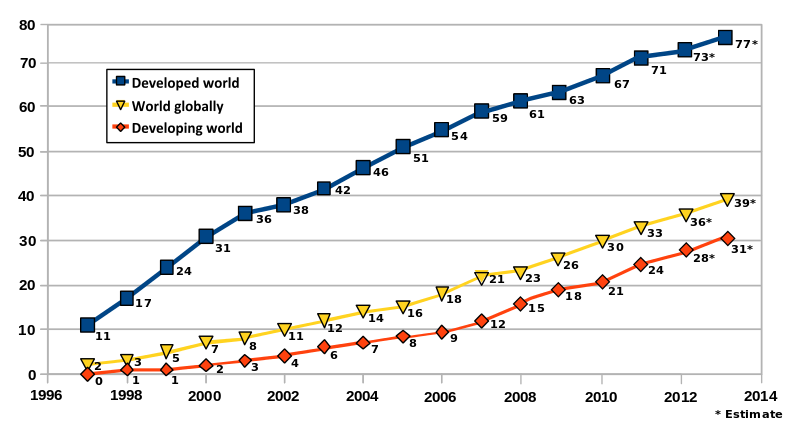
\includegraphics[width=15cm]{pictures/users.png}
  \caption{Počet uživatelů Internetu na 100 obyvatel ve světě. \newline(Příklad spojnicového grafu se třemi časovými řadami) \newline(Zdroj: <https://cs.wikipedia.org>)}
  \label{fig:řada}
\end{figure}

\normalsize\textbf{\newline Dekompozice časových řad}

Abychom mohli s časovou řadou pracovat, předpovídat budoucí hodnoty, dělat odhady (intervalové či bodové) apod., potřebujeme mít časovou řadu, která je alespoň stacionární, respektive slabě stacionární. Většina zkoumaných časových řad je nestacionární povahy. Ale často se nám správným očištěním (dekompozicí) řady může podařit, získat stacionární řadu. 

Většinou se předpokládá, že časová řada $y_t$ pro t = 1, 2, ..., T je sestavena z trendové, cyklické, sezónní a nesystematické složky.

\textit{Trendová složka} ($T_t$) je obecná dlouhodobá tendence vývoje zkoumaného jevu. Tato složka zachycuje stálé procesy působící během dlouhého období. Trend může mít rostoucí nebo klesající charakter a nebo může být časová řada bez trendu.

\textit{Cyklická složka} ($C_t$) popisuje jednotlivé periody (cykly) v hodnotách ukazatele časové řady. Taková kolísání se okolo trendu objevují během dlouhého období, tj. značně delší než jeden časový úsek časový řady. V těchto cyklech se střídají fáze růstu a poklesu. Délka a amplituda cyklické složky mohou být nepravidelné a mít měnící se charakter. Kvůli tomu, že tato složka působí dlouhodobě, je docela obtížné ji určit a popsat. 

\textit{Sezónní složka} ($S_t$) vyjadřuje stále se opakující odchylku trendu. Perioda této složky je mnohem menší než u složky cyklické. Takové výkyvy se objevují ve stejných obdobích kvůli obecně známým jevům.

Čtvrtou složkou časové řady je \textit{náhodná} neboli \textit{nesystematická složka} ($u_t$). \\ Náhodné procesy a chyby měření v datech jsou vyjadřeny pomocí této složky. 	

Existují dva typy dekompozice časových řad:

\begin{enumerate}

\item aditivní: hodnoty ukazatele časové řady jsou součtem hodnot jednotlivých složek
\begin{equation}
y_t = T_t + C_t + S_t + u_t
\end{equation}

\item multiplikativní: hodnoty ukazatele časové řady jsou součinem hodnot jednotlivých složek 
\begin{equation}
y_t = T_t \cdot C_t \cdot S_t \cdot u_t
\end{equation}

\end{enumerate}

Při aditivní dekompozici časové řady jsou jednotlivé složky uvažovány ve \\ stejných jednotkách jako hodnoty ukazatele příslušné časové řady. Předpokladem použití aditivní dekompozice je konstatní variabilita hodnot časové řady v čase.

V případě multiplikativní dekompozice má trendová složka stejné jednotky jako příslušná časová řada, ale ostatní složky zůstávají vyjadřeny relativně. Při takové dekompozici se variabilita časové řady v čase obvykle mění. Existuje několik důvodů pro využití dekompozice a odstranění jednotlivých složek časových řad:

\begin{itemize}
\item[a)] charakter vývoje, chování zkoumané řady lze odhalit z analýzy příslušných složek
\item[b)] sezónním očišt'ováním je možné odstranit výkyvy časové řady pro přehlednější zkoumání trendu
\item[c)] a nebo se dá odstranit trendová složka časové řady pro detailnější analýzu sezónnosti
\item[d)] dekompozice umožňuje provést předpověd' jednotlivých složek, což vede k lepšímu výsledku v předpovídání samotné časové řady; předpovědi složek se v takovém případě sečtou nebo vynásobí v závislosti na typu dekompozice
\end{itemize}

\subsection{Predikce}

Protože je tato práce zaměřena na predikci časových řad, je konstrukce předpovědí jednou z nejdůležitějších částí. Vhodná konstrukce předpovědí má velký význam pro dosažení lepších výsledků. V praktické části bude použit určitý model predikce, ale ještě předtím se v této kapitole zmíníme o některých jiných obecných aspektech, které jsou spojeny s předpovídáním časových řad. 

\textit{Bodová předpoved'} je hodnota představující nejpřesnější odhad budoucí hodnoty časové řady v jistém okamžiku. Tato hodnota je vždy zatížena určitou chybou, jejíž velikost záleží na vybraném modelu predikce. Pro úroveň přesnosti existuje pojem \textit{předpovědní interval}, který je analogií intervalu spolehlivosti v matematické statistice. Předpovědní interval tak určuje horní a dolní mez, mezi nimiž s určitou pravděpodoností leží predikovaná budoucí hodnota.  

Předpovědní metody se většinou rozdělují do dvou velkých skupin - \textit{kvalitativní} a \textit{kvantitativní}. Základem kvalitativních metod jsou názory expertů a odborníků v určité oblasti. Takové metody jsou použitelné v případě, kdy se zavádí nová technologie nebo zcela nový produkt a zatím neexistují žádná data. Dále jsou v práci prozkoumány a použity pouze kvantitativní předpovědní metody. Tyto metody jsou oproti kvalitativním založeny na analýze empirických dat. Analýza se provádí pomocí matematicko-statistického přístupu. Použití kvantitativních předpovědních metod předpokládá, že se s časem, kdy se provádí předpověd', charakter řady nemění. Tento fakt nemůžeme vynechávat a proto budeme zavádět drobná omezení v konstrukci předpovědní metody (např. rozdělení dat do intervalů s maximálně stejným vývojem). \cite{cipra}

V případě, že existují předem známá data a předpovědní metoda se určuje na základě těchto dat, hrají chyby v předpovědích a jejich minimalizace důležitou roli. Chyba je většinou definována jako rozdíl mezi reálnou hodnotou $y_t$ a predikovanou hodnotou $\hat{y_t}$, a zároveň je odhadem náhodné složky $u_t$:

\begin{equation}
e_t = y_t - \hat{y_t}
\end{equation}

Existují určité míry pro kontrolu kvality provedených předpovědí. Často se můžeme setkat s následujícími typy: 

\textit{Součet čtvercových chyb SSE} (Sum of Squared Errors):
\begin{equation}
\sum_{t=1}^{n}(y_t - \hat{y_t})^2 = \sum_{t=1}^{n}(e_t)^2
\end{equation}

\textit{Střední čtvercová chyba MSE} (Mean Squared Error)
\begin{equation}
\sum_{t=1}^{n}\frac{(y_t - \hat{y_t})^2}{n} = \sum_{t=1}^{n}\frac{(e_t)^2}{n}
\end{equation}

\textit{Střední absolutní odchylka MAD} (Mean Absolute Deviation)
\begin{equation}
\sum_{t=1}^{n}\frac{|y_t - \hat{y_t}|}{n} = \sum_{t=1}^{n}\frac{|e_t|}{n}
\end{equation}

\newpage
\section{Regresní analýza}
\vspace{0.5cm}

Regresní analýza je souhrnem statistických metod, používaných k matema-tickému popisu vztahu a závislosti jedné veličiny (závisle proměnná, vysvětlovaná proměnná neboli regresand) na jiné veličině (nezávisle proměnná, vysvětlující pro-měnná neboli regresor). Výsledkem regresní analýzy je informace o tom, jak se mění hodnota vysvětlované proměnné při změnách hodnoty vysvětlující proměnné. Tuto informaci pak můžeme využít pro predikci hodnoty vysvětlované proměnné pomocí regresní funkce. 

Regresní funkce se často používá pro odhad trendu časové řady, proto dále analýza regresní funkce a její parametrů bude považována za analýzu trendové funkce časové řady.

\subsection{Lineární regrese}

Pokud je regresní funkce lineární vzhledem k regresním koeficientům a vyjadřena vztahem 

\begin{equation}
\hat{y} = \sum_{j=1}^{k}b_jf_j(x),
\end{equation}

hovoříme o lineární regresní funkci, kde \textit{$b_j$} jsou regresní koeficienty a \textit{$f_j$}$(x)$ jsou předem známé funkce. Pomocí lineární regrese můžeme proložit soubor bodů v grafu přímkou či křivkou, v závislosti na typu vysvětlujícíh proměnných $x$. 

\begin{figure}[h]
  \centering
  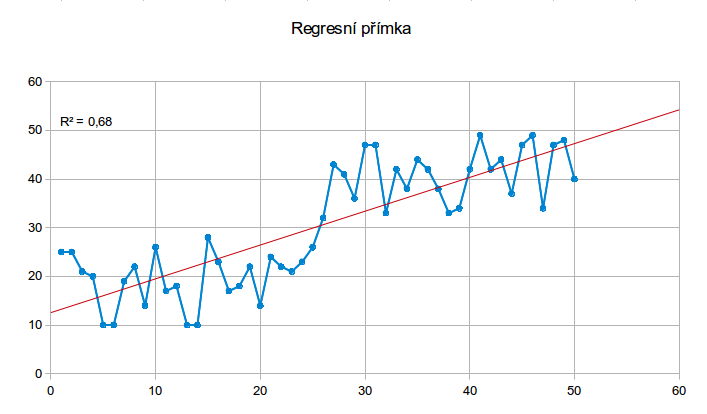
\includegraphics[width=15cm]{pictures/primka.png}
  \caption{Příklad proložení bodů v grafu regresní přímkou. \newline($R^2$ - koeficient determinace. Vlastní zdroj.)}
  \label{fig:přímka}
\end{figure}

V případě přímky (viz Obrázek 1.2) lineární regresní funkce má následující tvar

\begin{equation}
\hat{y} = b_0 + b_1x,
\end{equation}

kde $b_0$, $b_1$ jsou regresní koeficienty a $x$ je jedinou vysvětlující proměnnou. Regresní funkce je odhadem příslušného regresního modelu

\begin{equation}
y = \beta_0 + \beta_1x + e,
\end{equation}

kde $e$ je chyba mezi reálnou hodnotou $y$ a predikovanou hodnotou $\hat{y}$, pro kterou se předpokládá, že její střední hodnota je rovna nule, tj. $E(e) = 0$.

V komplikovanějším případě regresní funkce může být například mocninnou funkcí $\hat{y} = b_0 \cdot x^{b_1}$ nebo exponenciální $\hat{y} = b_0 \cdot b_1^x$. Tyto komplikace se řeší zloga-ritmováním příslušné rovnice. Zlogaritmováním pak dostáváme obě rovnice ve tvaru podobném rovnici (1.8), který můžeme zkoumat jako regresní funkci ve tvaru přímky.

\begin{figure}[h]
  \centering
  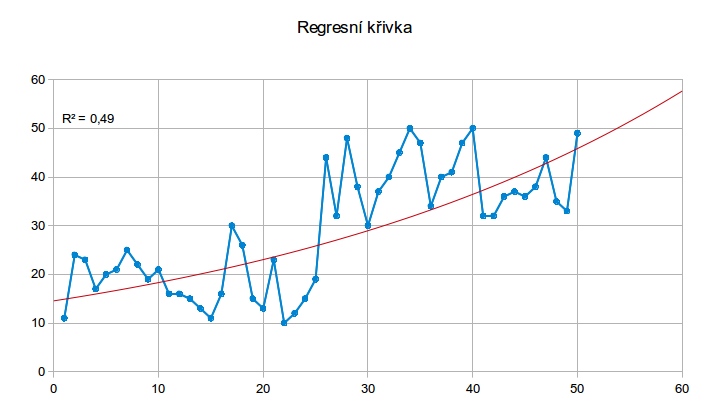
\includegraphics[width=15cm]{pictures/krivka.png}
  \caption{Příklad proložení bodů v grafu regresní exponenciální křivkou. \newline($R^2$ - koeficient determinace. Vlastní zdroj.)}
  \label{fig:křivka}
\end{figure}

Dalším zvláštním příkladem lineární regresní funkce je polynomická funkce. Úkolem se stává určit nejvhodnější regresní koeficienty polynomu stupně $k$, který nejlépe aproximuje zadané body

\begin{equation}
\hat{y} = P_k(x) = p_0 + p_1x + ... + p_kx^k,
\end{equation} 

kde koeficienty polynomu $p_0$, $p_1$ ... $p_k$ jsou koeficienty regresní polynomické funkce. 

Je ale pochopitelně, že přímka nebo křivka nemůže přesně procházet všemi danými body v grafu. Zatímco jsou x-ové souřadnice přesné, y-ové souřadnice regresní funkce obvykle zatíženy chybou (1.3). Proto potřebujeme využít metodu, pomocí které dokažeme určit nejoptimálnější hodnoty regresních koeficientů. 

\normalsize\textbf{\newline Metoda nejmenších čtverců}

Pro jednoznačnost výběru regresní funkce se nejčastěji používá \textit{metoda nejmenších čtverců} (OLS - Ordinary least squares), pro kterou platí, že součet čtverců odchylek je minimální

\begin{equation}
\sum_{t=1}^{n}(y_t - \hat{y_t})^2 = \sum_{t=1}^{n}(e_t)^2 \rightarrow min. 
\end{equation}

\begin{figure}[h]
  \centering
  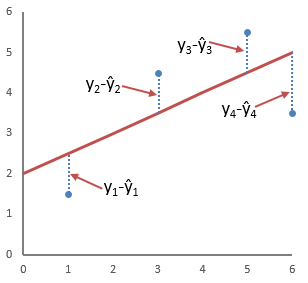
\includegraphics[width=8cm]{pictures/odchylky.png}
  \caption{Grafické znázornění odchylek. Zdroj: <http://exceltip.ru/>}
  \label{fig:odchylky}
\end{figure}

Ukažeme využití MNČ na výpočtu regresních koeficientů regresní funkce ve tvaru přímky, tj. ve tvaru (1.8). Minimalizujeme součet čtverců odchylek 

\begin{equation}
\sum_{t=1}^{n}(y_t - \hat{y_t})^2 = \sum_{t=1}^{n}(y_t - b_0 - b_1x)^2 \rightarrow min. 
\end{equation}

Přirovnáme parciální derivace podle parametrů $b_0$ a $b_1$ k nule a po úpravách získáme dvě rovnice

\begin{equation}
\sum_{t=1}^{n}y_t = nb_0 + b_1\sum_{t=1}^{n}x_t
\end{equation}

\begin{equation}
\sum_{t=1}^{n}y_tx_t = b_0\sum_{t=1}^{n}x_t + b_1\sum_{t=1}^{n}(x_t)^2
\end{equation}

Řešením těchto rovnic a dosazením daných hodnot $x_t$ a $y_t$, dostaneme hodnoty regresních koeficientů přímky

\begin{equation}
b_0 = \frac{\sum_{t=1}^{n}y_t\sum_{t=1}^{n}(x_t)^2 - \sum_{t=1}^{n}x_t\sum_{t=1}^{n}y_tx_t} {n\sum_{t=1}^{n}(x_t)^2 - (\sum_{t=1}^{n}x_t)^2} 
\end{equation}

\begin{equation}
b_1 = \frac{n\sum_{t=1}^{n}y_tx_t - \sum_{t=1}^{n}y_t\sum_{t=1}^{n}x_t} {n\sum_{t=1}^{n}(x_t)^2 - (\sum_{t=1}^{n}x_t)^2},
\end{equation}

kde $n$ je počet naměřených hodnot neboli pozorování. 

\subsection{Vícenásobná lineární regrese}

Sledování závislosti a vztahů mezi pouze dvěma proměnnými je v praxi velmi častým zjednodušením skutečnosti. Pro modely, které mají více než jednu nezá-vislou (vysvětlující) proměnnou, se využívá vícenásobná lineární regrese. Závislost vysvětlované proměnné v takovém případě je možno popsat regresní rovnicí 

\begin{equation}
\hat{y_t}(x) = b_0 + b_1x_{t1} + b_2x_{t2} + ... + b_kx_{tk},
\end{equation}

kde index $t$ značí jednotlivá pozorování a $k$ je počet regresorů (vysvětlujících proměnných). Daný model má jeden důležitý předpoklad, jehož podstatou je to, že libovolnou z nezávislých proměnných nemůžeme vyjadřit jako lineární kombinaci ostatních nezávislých proměnných. Jinak bychom nemohli jednoznačně určit regresní koeficienty, protože by mohlo existovat mnoho kombinací regresních koeficientů, které by vysvětlovaly veličinu $y$ se stejnou přesností. Tento problém se nazývá \textit{multikolinearita}, který se vyskytuje v důsledku korelace mezi vysvětlujícími proměnnými. V praxi se multikolinearita objevuje skoro v každém modelu.

Pro vícenásobnou regresní analýzu platí stejná metoda nejmenších čtverců, kterou taky můžeme popsat v maticovém tvaru 

$$
\begin{bmatrix}
\hat{y_1} \\
\hat{y_2} \\
\vdots \\
\hat{y_n}
\end{bmatrix}
=
\begin{bmatrix}
1 & x_{11} & x_{12} & \ldots & x_{1k} \\
1 & x_{21} & x_{22} & \ldots & x_{2k} \\
\vdots & \vdots & \vdots & \ddots & \vdots \\
1 & x_{n1} & x_{n2} & \ldots & x_{nk}
\end{bmatrix}
\cdot
\begin{bmatrix}
b_1 \\
b_2 \\
\vdots \\
b_k
\end{bmatrix}
$$

neboli 

\begin{equation}
\mathbf{y} = \mathbf{Xb}
\end{equation}

Po stejných úpravách pomocí parciálních derivací získáváme rovnici pro odhad vektoru regresních parametrů

\begin{equation}
\mathbf{b} = (\mathbf{X}^T\mathbf{X})^{-1}\mathbf{X}^T\mathbf{y}
\end{equation}

Jak již bylo řečeno, multikolinearita se do jisté míry vyskytuje v různých regresních modelech. Multikolinearita obecně ukazuje na závislost mezi vysvětlujícími proměnnými. Příčiny vyskytu mohou být následující

\begin{itemize}
\item přeurčený regresní model
\item pokud je matice vysvětlujících proměnných $\bf{X}$ singulární
\item špatná specifikace modelu
\end{itemize}

Důsledky multikolinearity

\begin{itemize}
\item velké standardní chyby
\item silná citlivost regresních koeficientů i na malé změny v datech
\item odhandnuté regresní parametry mohou být statisticky nevýznamné
\end{itemize}

V praxi můžeme multikolinearitu objevit z korelační matice, která je důležitým prvkem v korelační analýze. Míru závislosti obvykle popisujeme korelačním koeficientem. Nejčastěji se použivá párový (Pearsanův)korelační koeficient, který vyjadřen následujícím vztahem

\begin{equation}
\bf{R} = \frac{\sum_{t=1}^{n}(x_t - \bar{x})(y_t - \bar{y})}{\sqrt{\sum_{t=1}^{n}(x_t - \bar{x})^2\sum_{t=1}^{n}(y_i - \bar{y})^2}},
\end{equation}

kde jsou $\bar{x}$ a $\bar{y}$ příslušné stření hodnoty vysvětlující a vysvětlované proměnné. 

Hodnota korelačního koeficientu $\bf{R}$ je mezi -1 a +1. Orientačně pokud je $\bf{R}$ > 0.8, lineární závislost se považuje za silnou. 

Existují něktěré možnosti odstranění multikolinearity

\begin{itemize}
\item pro případ s přeurčeným regresním modelem můžeme vyřadit zbytečné vysvětlující proměnné, které určíme podle korelační matice  
\item zvětšení počtu pozorování
\item transformace pozorování - první diference, podíl proměnných
\end{itemize}

\normalsize\textbf{\newline Vhodnost modelu}  

Existuje hodně různých metod, pomocí kterých můžeme sestrojit model časové řady. Tyto metody se dají taky kombinovat. Proto je vždy mnoho možností, jakým způsobem zkoumat časovou řadu. V závislosti na vybrané metodě, můžeme dosáhnout různých výsledků. Posouzení těchto výsledku je důležitým procesem při určení vhodnosti modelu pomocí různých analytických mír.

\textit{Rozptyl} neboli \textit{střední kvadratická odchylka} je ukazatelem variability náhodné veličiny okolo její střední hodnoty. Z reálných empirických hodnot a vypočtených hodnot regresní funkce můžeme určit tři typy rozptylů

\begin{itemize}
\item rozptyl empirických hodnot $y$
\begin{equation}
s^{2}_y = \frac{1}{n}\sum_{t=1}^{n}(y_t - \bar{y})^2,
\end{equation}

tj. celkový součet čtverců (CSČ).

\item rozptyl vyrovnaných hodnot
\begin{equation}
s^{2}_{\hat{y}} = \frac{1}{n}\sum_{t=1}^{n}(\hat{y}_t - \bar{y})^2,
\end{equation}

tj. vysvětlený součet čtverců (VSČ).

\item reziduální rozptyl
\begin{equation}
s^{2}_{y-\hat{y}} = \frac{1}{n}\sum_{t=1}^{n}(y_t - \hat{y})^2,
\end{equation}

tj. nevysvětlený součet čtverců (NSČ).
\end{itemize}

Významným ukazatelem vhodnosti regresního modelu je koeficient determinace $\bf{R^2}$, který určíme jako podíl vysvětleného součtu čtverců na celkovém součtu ctverců

\begin{equation}
\mathbf{R^2} = \frac{\text{VSČ}}{\text{CSČ}} = 1 - \frac{\text{NSČ}}{\text{CSČ}} = 1 - \frac{e^Te}{y^Ty - n\bar{y}^2}
\end{equation}

a zároveň je druhou mocninou korelačního koeficientu $\bf{R}$. 

Koeficient determinace je vhodný ke statistickému testování modelu jako celku a nabývá hodnot z intervalu <0, 1>, kde případ $\bf{R}^2$=1 ukazuje na silnou závislost a vhodnost použití lineární regrese. \cite{fiala} 


\newpage
\section{Softwarová aplikace}
\subsection{Způsob realizace}

Po důkladném seznámení se s problematikou práce a s ní související teorií, byl stanoven způsob dosažení cílů práce, tj. způsob její praktické realizace. Tato realizace měla tři hlavní kroky:

\begin{enumerate}
\item Pomocí regresní a korelační analýzy zjistit určité parametry v datech, které nejméně nebo nejvíce ovlivňují závislé parametry, a jestli mezi sebou vůbec mají nějakou souvislost. 

\item Potom na základě těchto údajů, s uvážením výsledků regresní a korelační analýzy získat regresní model, který může být použitelný k predikci budoucích hodnot zkoumaného parametru. V daném případě jde o daný parametr \textit{Computation time} (z angl. doba trvání výpočtu), který vyvolává zatížení, jehož snížení je vlastně problematikou práce.

\item Posledním krokem je posouzení kvality výsledků.	
\end{enumerate}
 
Pro konstrukci aplikace je dán soubor dat skládající se z matice vysvětlujících promenných \textbf{X} a vektoru vysvětlovaných proměnných \textbf{y}. Protože je vysvětlovaná proměnná závislá na více než jedné vysvětlující proměnné, potřebujeme využít vícenásobnou lineární regresi. Pomocí korelační analýzy nejdřív zjistíme vzájemnou závislost mezi vysvětlujícími proměnnými. Na základě dosažených výsledků dokažeme řict, které jsou nezávisle proměnné pro nás významné nebo zbytečné. Uvidíme to z korelační matice, která popisuje závislosti mezi všemi proměnnými v modelu. 

Zároveň použijme metodu výběru nejlepší podmnožiny pro určení vysvětlujících parametrů s nejlepším koeficientem determinace. Metoda spočívá v tom, že z množiny všech vysvětlujících proměnných \{$x_1, x_2, ..., x_k$\} se vybírají kombinace (podmnožiny), pro které se vypočítá koeficient determinace. Podmnožina s nejlepším koeficientem determinace se pak bude použita pro odhad regresního modelu. Pomocí regresní analýzy pak dokažeme získat hodnoty regresních koeficientu, které mají větší vliv na chování závisle proměnné. 

\subsection{Základní předpoklady a nástroje}
Za výsledek této práce může být také považována softwarová aplikace, která by měla být užitečnou pomůckou pro dosažení cíle práce. Podstatou aplikace je načíst a zanalizovat datový soubor regresní metodou, poté použít dosažené výsledky pro získání regresního modelu a případně udělat predikci budoucích hodnot a vykreslit vývoj nejlépe predikovaných hodnot ve tvaru grafu časových řad. 

Jako programovací nástroj jsem vybral objektově orientovaný programovací jazyk \textit{Java}. Jedná se o populární a docela starý programovací jazyk jehož historie sahá do roku 1990, kdy ve firmě Sun Microsystems začali pracovat na jeho vytvoření. Na začátku to byl efektivní a jednoduchý jazyk určený pro spotřební elektroniku. S postupem času a s rostoucím užitím internetu se Java stala jedním z nejpoužívanějších programovacích jazyků ve světě. Hlavními důvody proč jsem zvolil pravě tento jazyk jsou: 

\begin{itemize}
\item výkonnost a jednoduchost syntaxe
\item široká použitelnost
\item přenositelnost a nezávislost na architektuře nebo na operačním systému
\end{itemize} 

Pro snadnější programatorskou práci se hojně využívá \textit{vývojové prostředí} neboli \textit{IDE} (IDE - \textit{Integrated Development Environment}). Je to soubor nástrojů pro přehlednější přístup ke zdrojovému kódu, ladění programů, hledání a opravu chyb a další užitečné věci pro programování. Vývojové prostředí se většinou skládá z textového editoru, kompilátoru a debuggeru. 

S programovacím jazykem Java se používá několik různých IDE. Liší se podle nabízených vlastností a možností. Pro svou práci jsem zvolil vývojové prostředí \textit{IntelliJ IDEA}. 

Pro lepší koordinaci se svým vedoucím jsem během práce použil webový nástroj \textit{GitHub}. Je to služba usnadňující spolupraci vývojářů, kteři používají verzovací nástroj Git. Využívá se pro sdílení a společnou práci na softwarových projektech. Tato služba poskytuje možnost sdílet a upravovat projekty jiných programatorů, což vede k lepším výsledkům a rychlejšímu ladění kódu. 

Jako nástroj pro správu, řízení a automatizaci tvorby aplikace jsem použil \textit{Apache}. I když je možné využit tento nástroj k psaní projektů v různých programovacích jazycích, podporován je převážně programovací jazyk Java. Maven se používá hlavně pro usnadnění práce při buildování programů a aplikací. Vývojové prostředí Intellij IDEA umožňuje pomocí nástroje Maven vytvořit programatorský projekt podle modelu \textit{Project Object Model}. Tento model určuje ze začátku kostru zdrojového kódu, závislosti na externích knihovnách a proces spouštění potřebných testů a podobně. Základ samotného nástroje Maven jsou pluginy, které běží pouze na příkazové řádce. 

K implementaci analytických metod bylo navrhnuto použít již existující knihovnu v jazyce Java, nebo si vytvořit vlastní. 

\chapter{Praktická část}
\section{Chybné pokusy}
\vspace{0.5cm}

Při výběru programovacích nástrojů byla uvažována možnost využití cizích, svobodně distribuovaných knihoven nebo frameworků vhodných pro práci s daty a případně pro jejich analýzu. Předpokladem pro pomocné nástroje byla jejich kompatibilita s programovacím jazykem Java. 

Knihovna je v programování soubor funkcí, procedur, datových typů a tříd, které slouží pro různé programy. Každá knihovna má své \textit{API} (z angl. \textit{application programming interface} - rozhraní pro programování aplikací). Pomocí kterého se určuje jakým způsobem jsou funkce z knihovny volány. Zatímco framework je softwarová struktura, která volá samotný kód uživatele. Framework může obsahovat vlastní procedury, podprogramy i knihovny. Framework nás ovšem může omezovat svoji pevnou strukturou a architekturou. 

Během hledání pomocných nástrojů a vhodných knihoven jsem našel dva zdroje, u kterých jsem předpokládal že by mohly zlepšit průběh práce. Po hlubším \\ prozkoumání se ukázalo že nejsou zas až tak vhodné pro náš projekt. Jednalo se především o velkou sbírku algoritmů pro práci s daty \textit{Weka} a framework \textit{Encog}.  
\vspace*{0.5cm}

\textbf{Weka}

Weka je populární balík programů, který slouží pro analýzu dat, modelování predikce a využívá se ve strojovém učení. Weka používá textové soubory s formátem ARFF (\textit{Attribute Relationship File Format}), který obsahuje atributy a jejich data. Weka má i grafické uživatelské rozhrání pro přehledný přístup k využití všech možností programu, což je velkou výhodou. Zaujalo mě taky to, že pomocí tohoto balíku by šlo snadno zvizualizovat výsledky analýzy. Na to má Weka vhodné nástroje a  proto může vykreslit graf časové řady s veškerými informacemi o jejím vývoji.

Tato sbírka nástrojů pro analýzu dat je napsaná v jazyce Java a proto jsem se rozhodl ji zkusit zapojit do programu a využít její možnosti. Hned zkraje jsem narazil na problém při konverzi CSV souboru do formátu ARFF, při kterém se vyskytovaly chyby v datech.

Po několika pokusech odstranit tyto chyby jsem zistil, že se zdrojový kód stává komplkovanějším a využití tohoto způsobu už nedává moc smysl. Proto hlavní důvod proč jsem odmítmul balík programů Weka, je nekompatibilita se strukturou kódu mého programu a ztěžování při konverzi a načítání datového souboru.            

\begin{figure}[h]
  \centering
  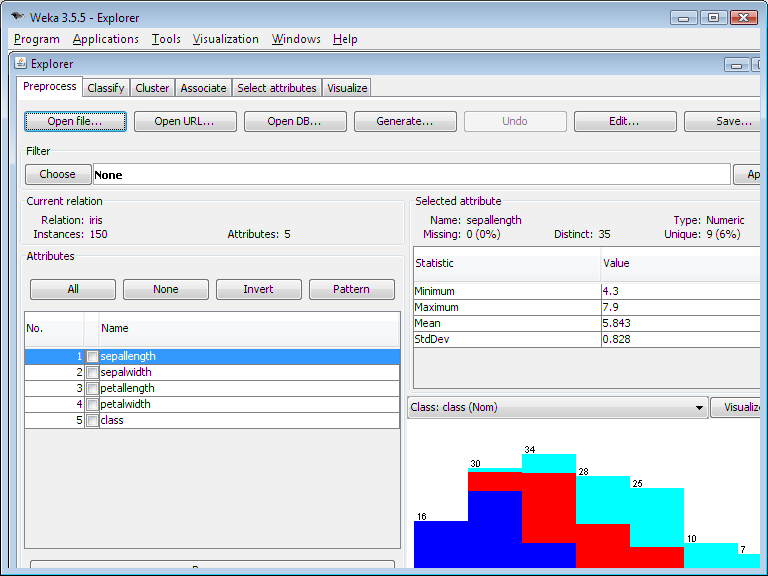
\includegraphics[width=15cm]{pictures/weka.png}
  \caption{Datový soubor otevřený v uživatelském rozhraní Weka \newline(Zdroj: https://cs.wikipedia.org)}
  \label{fig:weka}
\end{figure}

\newpage
\textbf{Encog}

Encog je framework pro strojové učení (z angl. \textit{Machine Learning}), což je oblast zabívající se algoritmy, které dávají strojům schopnost "učit se". Je to podoblast umělé inteligence (z angl. \textit{Artificial Intelligence}), která se používá pro studování inteligentního chování, adaptaci ve strojích, a také pro řízení, rozhodování a plánování procesů v různých systémech.

Tento framework zahrnuje pro problematiku této práce velmi užitečné techniky s regresními modely. Komplikace jeho využití byla v tom, že je vytvořen za použití neuronových sítí. Jak jsem později zjistil, ovládnutí těchto technologií pro mě bylo časově náročné a mimo oblast analytických metod, které jsem si na začátku stanovil. Kvůli tomu jsem se rozhodl zanechat tento nápad použití frameworku a hledat jiná řešení. 


\newpage
\section{Implementace}
\subsection{Datová vrstva}
Vzorová data se kterými pracují výpočetní servery, jsem dostal od svého vedoucího jako \textit{log file} (nebo taky \textit{žurnál}). Log je většinou textový soubor s příponou \textit{.log}, který obsahuje záznam činností nějakého programu nebo procesu. Tento záznam je ve tvaru posloupnosti jednotlivých kroků přislušného běhu programu, tj. skládá se z informací o tom jak, kdy, čím nebo kým byla využívána konkretní aplikace, jaké zatížení bylo vyvoláno nebo kolik času trvalo, aby příslušná aplikace proběhla. Logy se používají pro kontrolu procesů a zjištění přesné příčiny nějaké chyby, která nastala. Z jejich záznamů je možno určit co vedlo k chybě, jaký měla tato chyba vliv a jaké měl pak běžící proces důsledky. 

Daný soubor se skládá z dostatečně velkého množství řádků, v každém z nich je zaznamenávano několik parametrů. Tyto parametry obsahují vlastní hodnotu a/nebo jejich název. 

\begin{figure}[h]
  \centering
  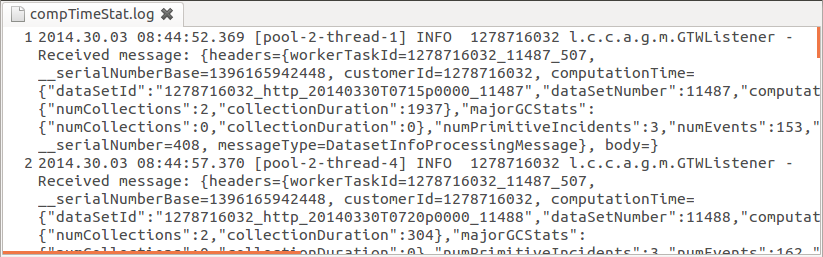
\includegraphics[width=15cm]{pictures/log.png}
  \caption{Log soubor (fragment). Vlastní zdroj.}
  \label{fig:log}
\end{figure}

Pro pohodlnější práci se souborem a odstranění nepotřebných parametrů (např. čas, datum) jsem se rozhodl překonvertovat log soubor do souborového formátu \textit{CSV} 	(z angl. \textit{comma-separated values}, neboli hodnoty oddělené čárkami). Je to jeden z nejednoduších formátů pro práci s tabulkovými daty. Považuji vybraný formát za vhodný, protože má podobnou strukturu jako log soubor a je často používán pro výměnu informací mezi různými systémy. Také je dost důležité, že se sloupce CSV souboru mohou tvářit jako časové řady, které se hojně využívají v regresní analýze.   

Pro konvertování log souboru do formátu CSV jsem použil \textit{shellový skript Bash}. Bash je jeden z unixových shellů, který interpretuje příkazový řádek. Shellové skripty jsou zápisem příkazů do souboru, které bychom jinak zadávali postupně na příkazovém řádku. Skript lze snadno spustit a vykonávat jím opakovanou činnost. Ty-picky se shellové skripty používají na unixových platformách, ale používají se též na Microsoft Windows.

\begin{figure}[h]
  \centering
  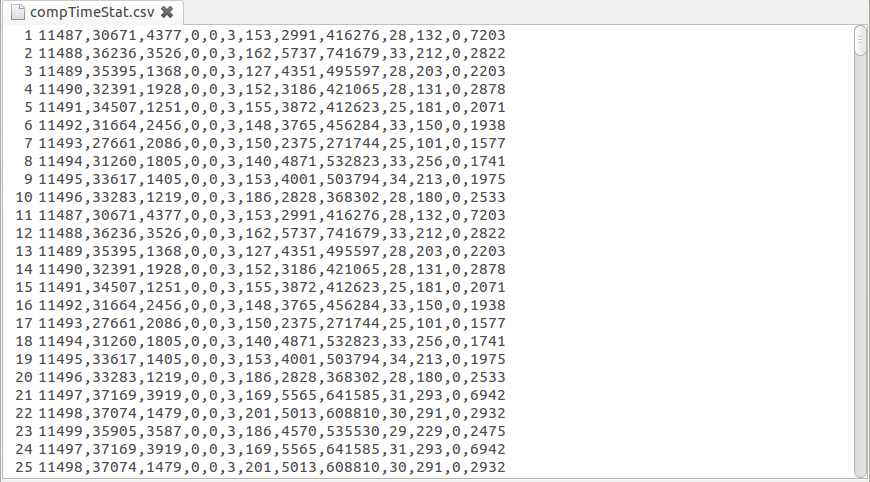
\includegraphics[width=15cm]{pictures/csv.png}
  \caption{CSV soubor (fragment). Vlastní zdroj.}
  \label{fig:csv}
\end{figure}

\newpage
\subsection{Aplikační vrstva}

Projekt vytvořený pomocí spravovacího nástroje Maven obvykle má následující adresářovou strukturu
\vspace*{0.5cm}

\begin{tabular}{|l|p{10cm}|}
  \hline
  {\bf Adresář} & {\bf Popis} \\
  \hline \hline
  Kořenový adresář        & obsahuje pom.xml ostatní adresáře \\
  \hline
  src/main/java     & obsahuje kompilovatelné .java soubory \\
  \hline
  src/main/resources    & obsahuje další soubory, například konfigurační XML \\
  \hline
  src/test/java          & obsahuje třídy testů \\
  \hline
  src/test/resources        & obsahuje konfigurační soubory pro testy \\
  \hline
\end{tabular}

V mém případě je pouze obsazená adresář src/main/java. I když testování je velmi dobrou praktikou mnoha programatorů, ja jsem se testy zdrojového kódu v dané práci nezabýval. 

Celý program se skládá ze tří tříd: 

\begin{enumerate}
\item \begin{lstlisting}
com.bp.prediction.oldClasses.ReadData.java
\end{lstlisting}

Daná třída byla vytvořena pro načítání dat. Jak již bylo zmíněno, pro vytvoření programu byl použit datový soubor \textit{Data.csv}, proto byl využit externí balíček na práci s CSV soubory pomocí

\begin{lstlisting}
import au.com.bytecode.opencsv.CSVReader;
\end{lstlisting}

Následně se tento soubor stal maticí z vysvětlujících a vysvětlované proměnné. 

\item \begin{lstlisting}
com.bp.prediction.oldClasses.NumberPrediction.java
\end{lstlisting}

V této třídě se prováděly hlavní procedury a vypočty. Obsahuje tato třída několik různých metod. 
První z nich je metoda pro převedení souboru dat do matice v příslušné třídě:

\begin{lstlisting}
public List<String[]> createMatrix()
\end{lstlisting}

Další metoda rozděluje matici dat do matice vysvětlujících proměnných \textit{xData} a do vektoru hodnot vysvětlované proměnné \textit{yData}:

\begin{lstlisting}
void fillMatrix(int[] xParameters) 
\end{lstlisting}

Potom je tam metoda pro využití korelační analýzy. Výstupem je pole hodnot koeficientů determinace všech kombinací, vytvořených z podmnožin množiny vysvětlujících proměnných:

\begin{lstlisting}
double[] getRSquaredStatistics(ArrayList<int[]> list)
\end{lstlisting}

Pro vytvoření kombinací v předchozí metodě napsal jsem dvě metody využívajících rekurze:

\begin{lstlisting}
static void permutation(int pos, int maxUsed) 
ArrayList<int[]> getCombinations() 
\end{lstlisting}

Poslední metodou v této třídě je metoda pro zjištění regresních koeficientů:

\begin{lstlisting}
double[] regressionParameters(int[] bestParameters)
\end{lstlisting}


\item \begin{lstlisting}
com.bp.prediction.oldClasses.GraphDrawing.java
\end{lstlisting}

Tato třída byla využita pro nakreslení vývoje zkoumané časové řady a odhadnuté regresní přímky. 
\end{enumerate}

\newpage
\section{Testování aplikace}
\subsection{Testovací data}

Jako testovací data jsem měl soubor dat ve formátu CSV. Tento soubor dat popisující určitý proces se skládá z osmi nezávisle proměnných a jedné závisle proměnné: 

$ \\
x_1 - dataSetNumber \\
x_2 - numFlows \\
x_3 - flowLoadingTime \\
x_4 - numEvents \\
x_5 - numFlowsInEvents \\
x_6 - resultSize \\
x_7 - numArtificialFileDownloadEvents \\
x_8 - numFileDownloadFlows \\ \\
x_9 = y - computationTime
$ 
\subsection{Zpracování a analýza dat}

\normalsize\textbf{\newline Korelační matice} 

Jako první metoda analýzy, kterou program spouští je korelační matice všech proměnných. Pro přehled jsem vytvořil trojuhelnikovou korelační matici

$$
\begin{bmatrix}
x_1 & 1.000\\
x_2 & 0,847 & 1,000\\
x_3 & 0,721 & 0,820 & 1,000\\
x_4 & 0,832 & 0,958 & 0,777 & 1,000 \\
x_5 & 0,802 & 0,981 & 0,827 & 0,920 & 1,000 \\
x_6 & 0,805 & 0,981 & 0,821 &0,925 & 0,999 & 1,000 \\
x_7 & 0,849 & 0,991 & 0,828 & 0,944 & 0,987 & 0,988 & 1,000 \\
x_8 & 0,811 & 0,955 & 0,807 & 0,909 & 0,954 & 0,955 & 0,958 & 1,000 \\
y & 0,774 & 0,806 & 0,802 & 0,786 & 0,781 & 0,786 & 0,800 & 0,786 & 1,000 
\end{bmatrix}
$$

Z analýzy korelačních koeficientu matrice je vidět, že je v těchto datech multikolinearita. Vyloučením zbytečných vysvětlujících proměnných jsem dostal korelační matici z dvěma vysvětlujícími proměnnými $x_3$ a $x_4$ a jednou vysvětlovanou proměnnou $y$.   

Následně jsem vypočital koeficient determinace a přislušné regresní koeficienty pro tento změnšený model pomocí příslušných tříd: 

\begin{displaymath}
\begin{array}{ll}
R^2 = 0.7101 \\
b_0 = 3430.5582, b_1 = 0.5897, b_2 = 6.1441
\end{array}
\end{displaymath}

\normalsize\textbf{\newline Metoda výběru nejlepší podmnožiny}

Výsledkem metody výběru nejlepší podmnožiny se stala samá množina všech vysvětlujících proměnných, tj. ${x_1, x_2, x_3, x_4, x_5, x_6, x_7, x_8}$. Jejím koeficientem determinace je hodnota $R^2 = 0,7616$. Však my tuto metodu musíme zamítnout kvůli silné multikolinearitě.  

\subsection{Vizualizace}

Pro realizaci dosažených výsledků bychom měli nejdřív sestavit regresní odhadovou funkci a pak nakreslit tuto přímku. Přímka je v dané, případě lineárním odhadem trendové funkce zkoumané časové řady. Pro regresní funkci platí

\begin{equation}
\hat{y} = 3430.5582 + 0.5897x_3 + 6.1441x_4
\end{equation}

Pomocí třídy \textit{com.bp.prediction.oldClasses.GraphDrawing.java} dostáváme graf popisující vývoj časové řady a její odhadnutý trend.

\begin{figure}[h]
  \centering
  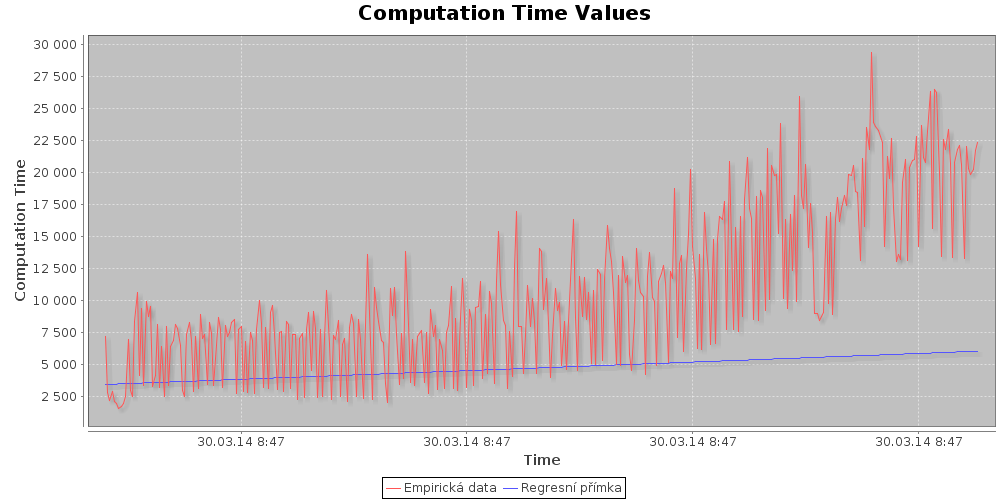
\includegraphics[width=15cm]{pictures/regresniFunkce.png}
  \caption{Graf vývoje časové řady a trendu \newline(Součástí výstupu programu)}
  \label{fig:regrese}
\end{figure}

Statistickou významnost modelu jako celku podle koeficientu determinace, lze testovat podle testovacího kritéria 

\begin{equation}
F = \frac{R^2}{1 - R^2}\frac{n-(k+1)}{k},
\end{equation}

které má Fisherovo rozdělení s $k$ a $n-(k+1)$ stupni volnosti $F[k, n-(k+1)]$. 

\newpage
Nulová a alternativní hypotézy:

\begin{itemize}
\item $H_0$: statistická nevýznamnost $R^2$
\item $H_A$: statistická významnost $R^2$
\end{itemize} 

Poduk platí $F > F*$, odmítáme hypotézu $H_0$ a znamená to, že hodnota $R^2$ je statisticky významná a ne všechny regresní parametry jsou rovny nule. 

Jestliže platí $F < F*$, akceptujeme hypotézu $H_A$ o statistické nevýznamnosti $R^2$. To znamená, že vysvětlující proměnné neovlivňují významně vysvětlovanou proměnnou a všechny regresní parametry jsou nulové.

V tomto případě pro Fisherovo rozdělení platí $k = 2$, $n-(k+1) = 384$. Pak \space\space\space $F$ = 195,28 a $F*$ = 470,34. Odsud vyplývá, že $F < F*$ a akceptujeme hypotézu $H_0$, tj. koeficient determinace $R^2$ je statisticky nevýznamný.  
 


\chapter*{Závěr}
\addcontentsline{toc}{chapter}{Závěr} % SEM NESAHEJTE!

Základním cílem této bakalářské práce bylo navrhnout počítačovou aplikaci, která by pomocí regresní a korelační analýzy mohla zjistit závislost nebo nezávislost mezi hodnotami v určitých souborech dat. Po využití analytických metod a jejich implementování v programu, byly získány výsledky odhadu regresního modelu. Z grafu ukazujícího odhadnutý trend a z výsledku testování je evidentně, že odhadnutý model není dostatečně významný. Popis trendu časové řady matematickými křivkami je častým způsobem v analýze časových řad. Použil jsem dvě metody pro řešení vícenásobné lineární regrese. 

První je metoda výběru podmnožiny s nejlepším koeficientem determinace. Ukázala tato metoda, že nejlepší podmnožina pro odhad regresního modelu je samá množina se všemi proměnnými. Z korelační matice ale vidíme, že jsou v tomto modelu silné závislosti mezi mnoha vysvětlujícími proměnnými. Proto jsem musel postoupit k druhé metodě. 

Druhá metoda je založena na analýze korelační matice. Korelační matice může popisovat závislosti mezi úplně všemi proměnnými v modelu a může takovým způsobem objevit multikolinearitu, což je zbytečná závislost mezi vysvětlujícími proměnnými. Kvůli výskytu silné multikolinearity bylo potřeba vyřadit zbytečné nezávislé proměnné. Po takovém vyloučení zbylo jen dvě vysvětlující proměnné, jejichž koeficient determinace jsem následně analyzoval. Testování významnosti koeficientu determinace ukázalo, že i tyto dvě proměnné významně neovlivňují vysvětlovanou hodnotu. 

Pro implementaci potřebných analytických metod byla navrhnuta aplikace. I když architektura vytvořeného programu není výborná, běh programu je dostatečně rychlý. Program obsahuje třídy s pouze základními metodami pro analýzu regresních modelů. Je možné přidat hodně různých metod pro analýzu a testování regresních modelu. Taky by bylo užitečné v budoucnu přidat třídu pro analýzu nelineárních regresních modelu. Jako další možné zlepšení aplikace je přidání metod regresní analýzy popisující nelineární trend. Tyto metody jsou možným řešením nalezení regresního modelu pro uvedený v této práci soubor dat. 

Z programovacího pohledu, kvalita zdrojového kódu se taky může zlepšit. Zatím byly použity jednoduché algoritmy a využity externí knihovny. Uživatelské rozhraní by bylo vhodným pro ty kteří se dobře nevyznají v programování. I když v programu není zatím uživatelské rozhraní, pro programatora je docela jednoduché se rozebrat v konstrukci programu. 

V závěru jsem popsal použité postupy pro dosažení staveného cíle a jeich výsledky. Taky jsem uvedl možná rozšíření programu. 

\clearpage
\addcontentsline{toc}{chapter}{Literatura} % SEM NESAHEJTE!
\begin{thebibliography}{99}   
	\bibitem FFumio Hayashi. \emph{Econometrics}. Princeton. Princeton University Press, 2000. ISBN 9780691010182.
	\bibitem{cipra} Tomáš Cipra. \emph{Analýza časových řad s aplikacemi v ekonomii}. Praha. SNTL - Nakladatelství technické literatury, 1986.
	\bibitem{fiala} Petr Fiala. \emph{Úvod do ekonometrie}. Praha. Nakladatelství ČVUT, 2008. \\ ISBN 978-80-01-04004-1
	\bibitem{arlt} Josef Arlt, Markéta Arltová, Eva Rublíková. \emph{Analýza ekonomických časových řad s příklady}. Skripta VŠE Praha, 2002. ISBN 80-245-0307-7. V elektronické podobě k dispozici na <http://kstp.vse.cz/o-katedre/clenove-katedry/marketa-arltova/>
	\bibitem PPoužitá Java dokumentace. URL: <http://commons.apache.org/proper/commons-math/apidocs/org/apache/commons/math3/stat/regression/> 	
	
\end{thebibliography}

\newpage % SEM NESAHEJTE!
\addcontentsline{toc}{chapter}{Přílohy} % SEM NESAHEJTE!
\appendix % SEM NESAHEJTE!

\chapter{Uživatelská příručka} % SEM NESAHEJTE!

Výslednou aplikací se v této práci rozumí zdrojový kód, který slouží pro analýzu souboru dat. Pro jeho správné a spolehlivé použití uživatel musí mít naistalované vývojové prostředí Intellij IDEA verze 13.1.6, protože zdrojový kód byl vytvořen pomocí spravovacího nástroje Maven, který přidává aplikaci určitou konstrukci. 

Po otevření programu v Intellij IDEA by uživatel měl nejdřív importovat závislosti nástroje Maven. Tyto závislosti způsobují stažení a využití externích knihoven, potřebných pro příslušné metody. Jednotlivé závislosti se správují v souboru \textit{pom.xml}. 

V třídě \textit{com.bp.prediction.oldClasses.ReadData.java} se nastavuje jmeno zkoumaného souboru dat, který se musí nacházet v adresáři \textit{/com.bp.prediction.oldClasses.NumberPrediction/}. Při změně souboru dat se musí taky v třídě změnit předdefinovaná hodnota \textit{xParams} určující počet nezávisle proměnných v modelu.

Pro analýzu souboru dat se musí spustit třída \textit{com.bp.prediction.oldClasses.NumberPrediction.java}, která obsahuje metodu \textit{public static void main(String[] args)}.

Uživatel by pak měl dostat ve výstupu (předpokládá se využití testovacího souboru \textit{Data.csv}):

\begin{itemize}
\item vypsána korelační matici 
\item obrázek s vývojem časové řady a odhadnutého trendu
\item textový výstup ve tvaru:

\textit{Metoda výběru nejlepší podmnožiny:} \\
\textit{Nejlepší koeficient determinace = 0,7616} \\
\textit{Vysvětlující proměnné:} \\
$x_1 x_2 x_3 x_4 x_5 x_6 x_7 x_8$

\textit{Určení koeficientů podle korelační matice:} \\
\textit{Nejlepší vysvětlující proměnné podle korelační matice:} $x_3, x_4$ \\
\textit{Regresní koeficienty nejlepších vysvětlujících proměnných:} \\
$b_0 = 3430.5582520692515 b_1 = 0.5897176399280367 b_2 = 6.144125208268643$
\end{itemize}

\chapter{Obsah přiloženého DVD}

\begin{itemize}
\item bakalářská práce ve formátu PDF
\item zdrojový kód aplikace
\end{itemize}

\end{document} % SEM NESAHEJTE!
